\label {fs-experiments}

\begin{figure}[htbp]
  \centering
  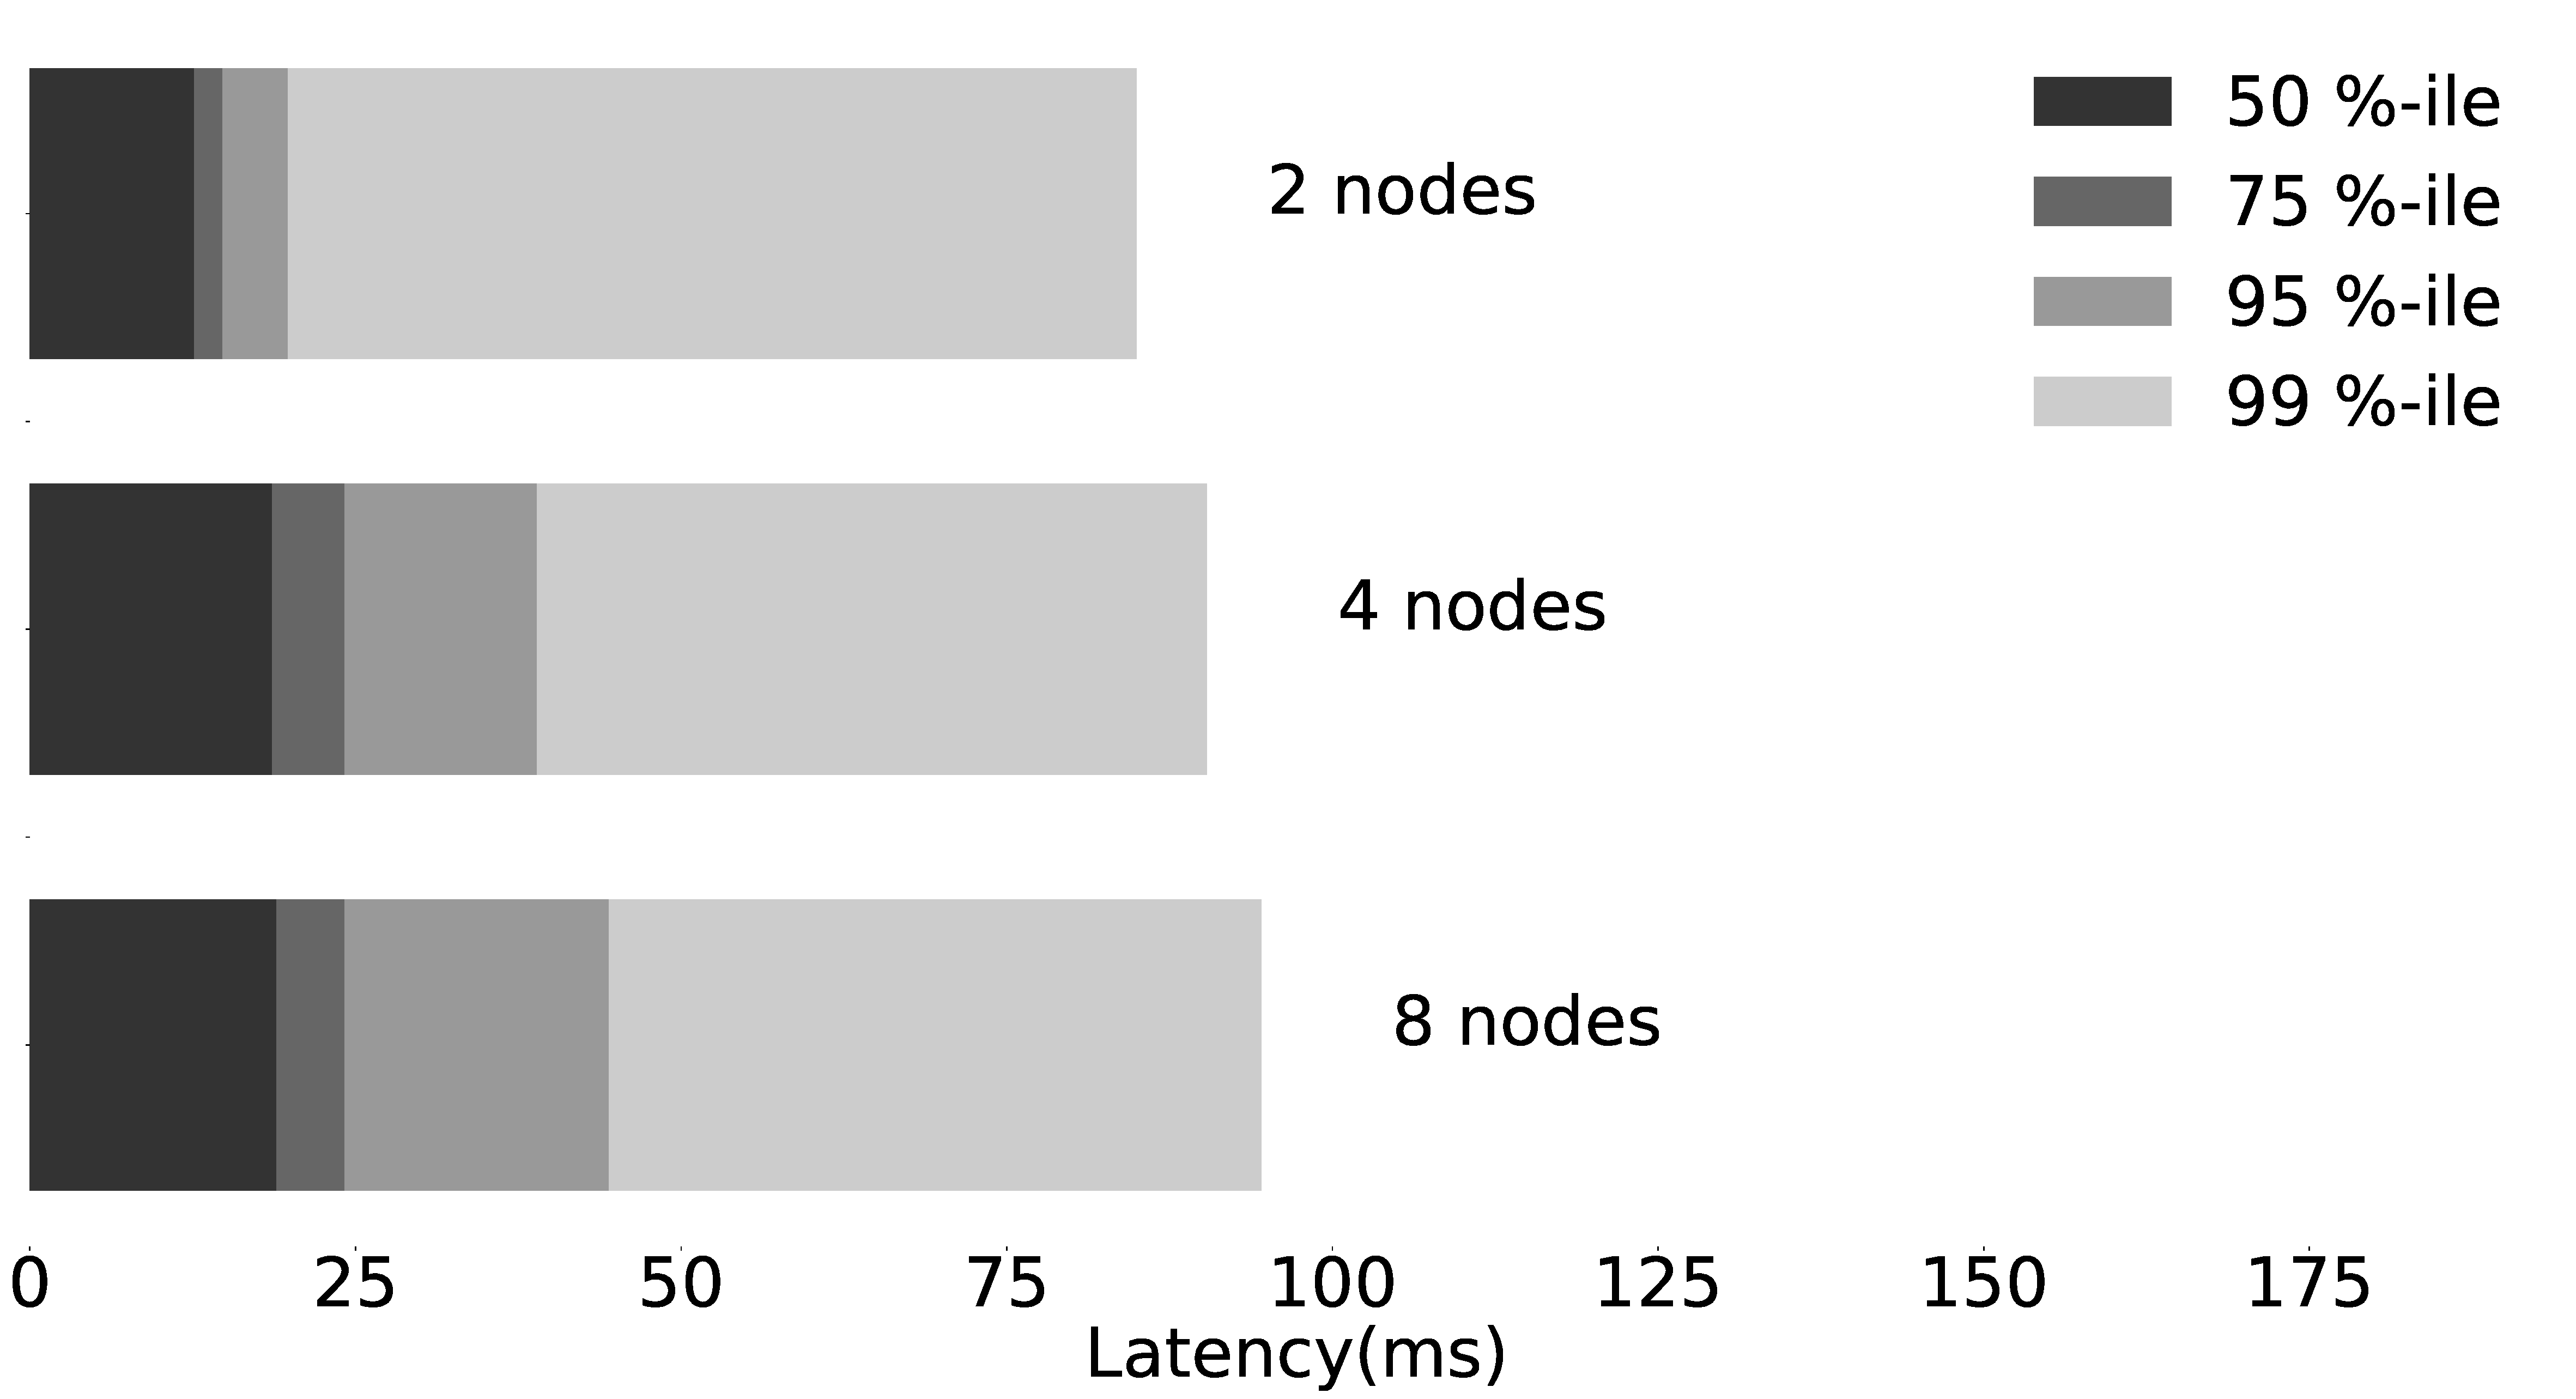
\includegraphics[scale=0.1]{pics/classifier_latencies}
  \caption{Classifier latencies}
  \label {latencies}
\end{figure}

To prove the feasibility of our pipeline we conducted series of experiments. As the dataset, we used russian news articles provided by lenta.ru. The dataset contains about 700 000 documents, which labeled by about 90 different kinds of topics. 

We deployed FlameStream on different clusters, containing 2, 4 and 8 nodes respectively. These nodes are Amazon AC2 small nodes with 2 GB of RAM and 1 core CPU. The results are shown in Figure ~\ref{latencies} and ~\ref{throughput}. There is a linear trend in performance, which proves the scalability of our pipeline. On the other hand, we can observe, that mean latency of classifier prediction have a slight increase. For each deployment the median is less then 25 ms and 99 percentile is less that 100 ms, which is reasonable result for the deterministic system with exactly-once support.

\begin{figure}[htbp]
  \centering
  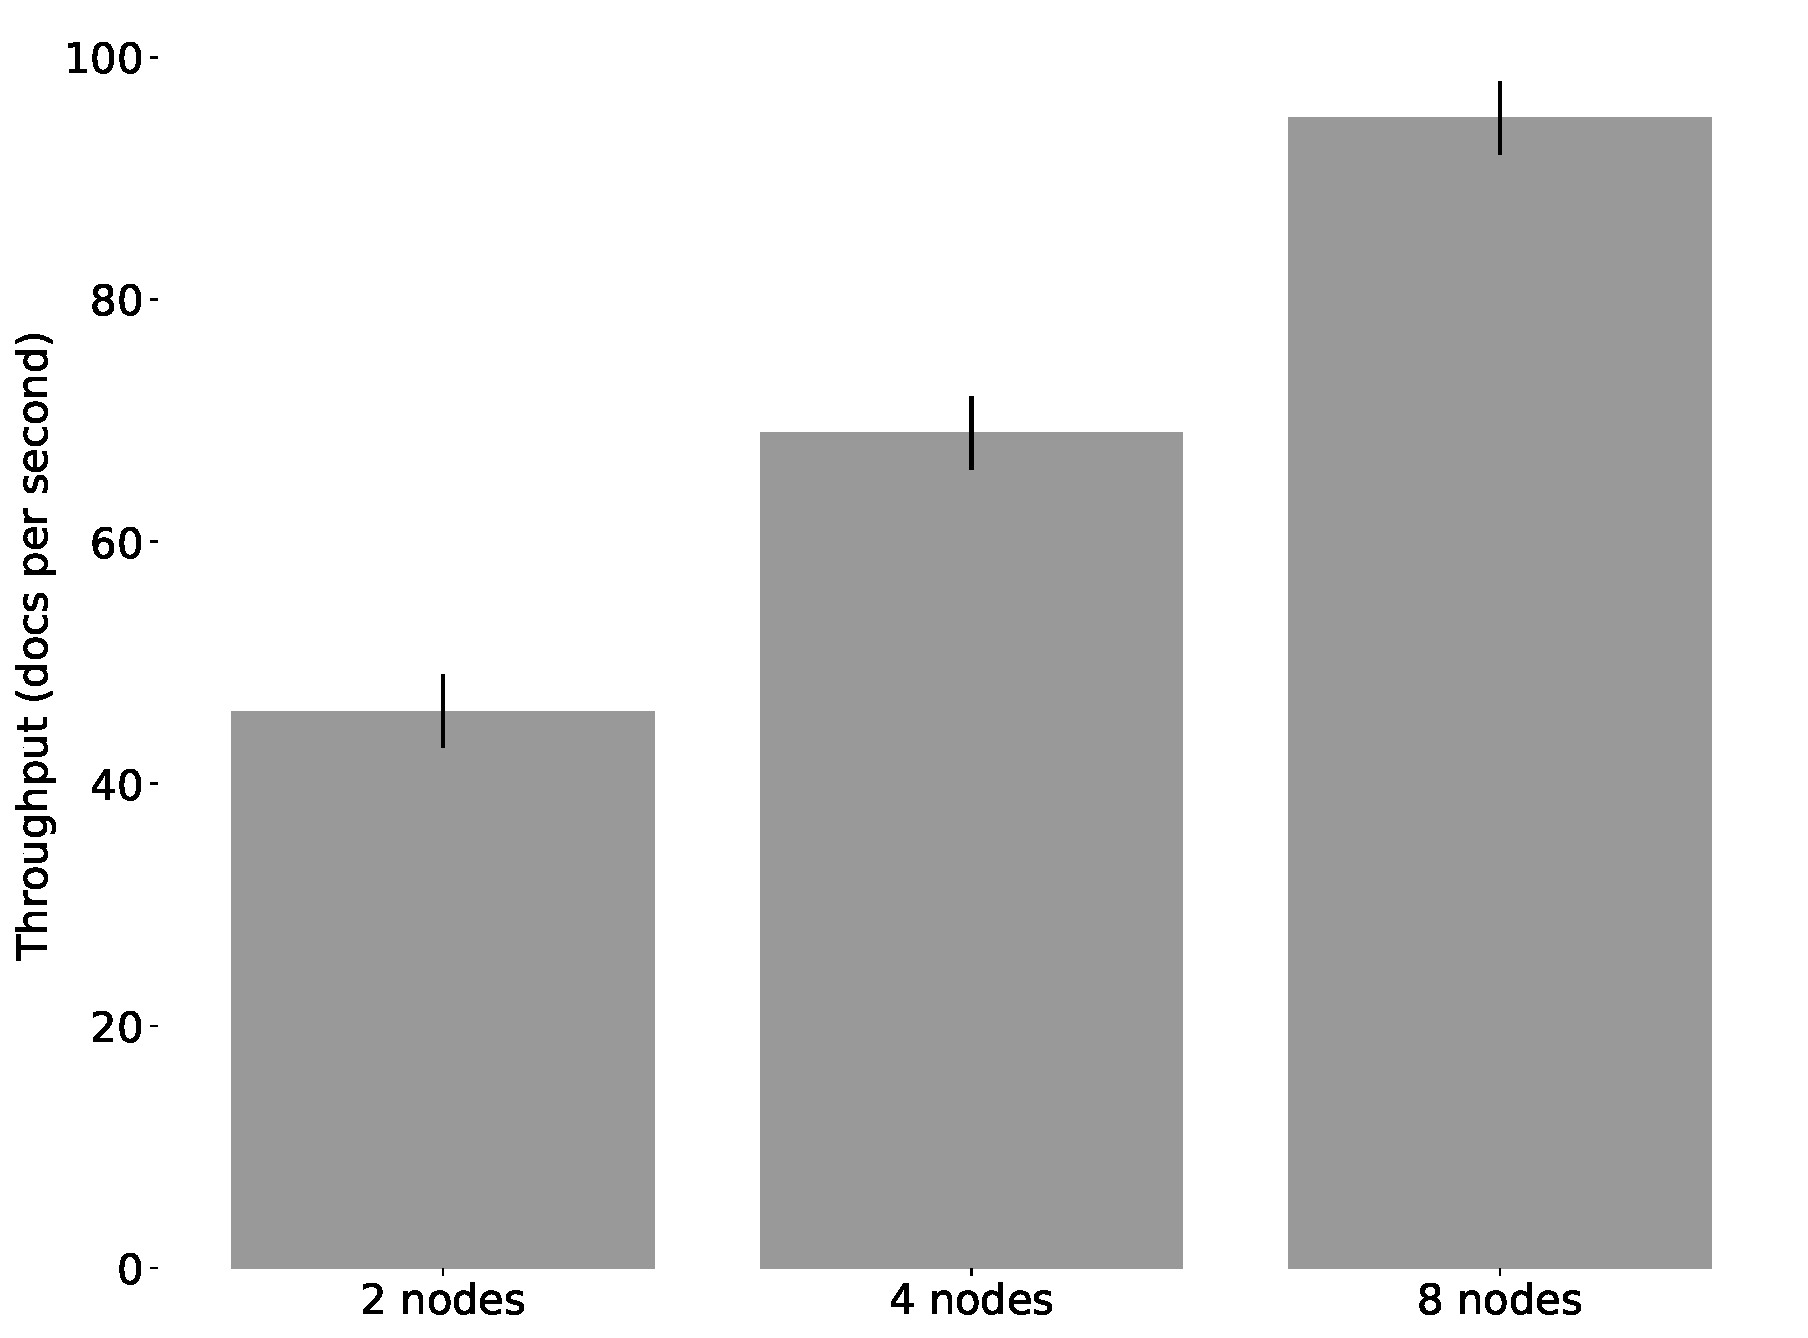
\includegraphics[scale=0.2]{pics/classifier_throughput}
  \caption{Classifier throughput}
  \label {throughput}
\end{figure}